\documentclass[11pt]{article}

% --- Packages ---
\usepackage[margin=1in]{geometry}
\usepackage{graphicx}
\usepackage{booktabs}
\usepackage{amsmath,amssymb}
\usepackage{hyperref}
\usepackage{xcolor}
\usepackage{enumitem}
\usepackage{caption}
\usepackage{subcaption}
\usepackage[T1]{fontenc}
\usepackage{microtype}
\usepackage{listings}
\usepackage{natbib}
\bibliographystyle{plainnat}

\hypersetup{
    colorlinks=true,
    linkcolor=blue!60!black,
    citecolor=green!50!black,
    urlcolor=blue!70!black,
}

\lstset{
    basicstyle=\ttfamily\small,
    breaklines=true,
    frame=single,
    backgroundcolor=\color{gray!5},
}

\title{\textbf{BF16 Precision Limits in Iterative Neural Architectures\\on AMD XDNA2 NPU}}

\author{
    % Your name here \\
    % Affiliation \\
    % \texttt{email@example.com}
}

\date{}

\begin{document}
\maketitle

% ============================================================
\begin{abstract}
Neural Processing Units (NPUs) in consumer processors promise efficient on-device AI inference through low-precision matrix units, but their numerical limitations remain poorly characterized for iterative architectures. We present the first bare-metal characterization of BF16 precision through an iterative weight-sharing architecture---the ALBERT encoder in Kokoro TTS---on AMD XDNA2 (AIE2P) hardware. Using the IRON close-to-metal programming framework, we bypass the vendor auto-partitioning toolchain (which fragments Kokoro into 36 CPU--NPU subgraphs with zero speedup) and achieve 1.31$\times$ speedup over CPU (229\,ms vs.\ 300\,ms for 12 ALBERT passes). However, we find that BF16 input truncation in the hardware matrix unit (\texttt{aie::mmul}) compounds through 12 iterative passes via correlated error amplification, degrading Pearson correlation from 0.9993 (single pass) to 0.698 (full NPU) or 0.974 (best hybrid). Even at 0.974 correlation, the downstream duration predictor produces different phoneme timings, yielding audio with 11.3\% duration mismatch and $-10.5$\,dB SNR---functionally unusable. We isolate three error sources (BF16 storage, GEMM input truncation, MHA block quantization) and show that MHA accounts for 80\% of precision loss while GEMM truncation creates an irreducible 0.974 ceiling. INT8 quantization via AMD Quark produces even worse results ($-15.6$\,dB SNR). Our findings establish that BF16-only matrix units are fundamentally incompatible with iterative weight-sharing at depth $\geq$12, with implications for deploying diffusion models, Universal Transformers, and other iterative architectures on current-generation NPU hardware.
\end{abstract}

% ============================================================
\section{Introduction}

Neural Processing Units are proliferating across consumer hardware. AMD's XDNA2 NPU (branded Ryzen AI) ships in every Ryzen AI 300-series processor, offering 50\,TOPS INT8 and 14.7\,TFLOPS BF16 through a $4\times8$ array of AI Engine tiles. Intel's Meteor Lake and Qualcomm's Hexagon include similar dedicated accelerators. The promise is clear: efficient, low-power inference for always-on AI workloads without taxing the CPU or GPU.

These NPUs achieve high throughput through reduced-precision arithmetic. AMD's AIE2P tiles provide an \texttt{aie::mmul} intrinsic that accepts only BF16 (bfloat16) inputs---8-bit exponent, 7-bit mantissa, approximately 3.9 decimal digits of precision. FP32 accumulation is available during the multiply-accumulate operation, but operand inputs are irrecoverably truncated. For single-pass architectures (standard transformers, CNNs), this truncation is well-tolerated: each layer's error is small and largely uncorrelated with subsequent layers' errors.

However, a growing class of neural architectures reuse the same weights iteratively. ALBERT~\citep{lan2020albert} applies a single shared transformer layer $N$ times in sequence, feeding each pass's output back as the next pass's input. Diffusion models~\citep{ho2020denoising} apply a shared UNet through 16--50 denoising steps. Universal Transformers~\citep{dehghani2019universal} iterate until convergence. In these architectures, BF16 truncation errors do not stay independent---they feed back through the same weight matrices, creating correlated error amplification.

We investigate this interaction empirically using Kokoro TTS~\citep{kokoro2024}, an 82M-parameter text-to-speech model with an ALBERT encoder (1 shared transformer layer, 12 passes, hidden dimension 768) followed by LSTM duration predictors, a convolutional decoder, and a HiFi-GAN vocoder. We program the AMD XDNA2 NPU at the bare-metal level using MLIR-AIE and IRON~\citep{iron2024}, bypassing the vendor VitisAI auto-partitioning toolchain which produces 36 CPU--NPU subgraphs with no measurable speedup.

\paragraph{Contributions.}
\begin{enumerate}[nosep]
    \item We demonstrate that BF16 input truncation compounds through iterative weight-sharing, producing correlation degradation from 0.9993 to 0.698 across 12 passes.
    \item We isolate three independent error sources and quantify their contributions.
    \item We show that even the best hybrid configuration (0.974 correlation) fails a sensitive downstream consumer (duration prediction), despite appearing numerically adequate.
    \item We provide the first bare-metal XDNA2 performance characterization for a complete transformer workload, achieving 229\,ms through 6 optimization steps from an initial 1022\,ms.
    \item We establish practical guidelines for deploying iterative architectures on BF16-only accelerators.
\end{enumerate}

% ============================================================
\section{Background}

\subsection{AMD XDNA2 Architecture}

The AMD XDNA2 NPU (codenamed Strix) integrates an array of AI Engine 2P (AIE2P) tiles. Each tile contains a vector processor with a hardware matrix multiply unit accessed through the \texttt{aie::mmul<M,K,N>} intrinsic. For BF16, the supported shape is \texttt{aie::mmul<4,8,8>}, processing a $4\times8$ BF16 matrix multiplied by an $8\times8$ BF16 matrix per cycle. The \texttt{prio\_accuracy} mode enables FP32 accumulation within the multiply-accumulate pipeline, but input operands are still truncated to BF16 before multiplication.

The NPU communicates with the host via DDR through a shim DMA layer. Kernel dispatch uses the Xilinx XRT runtime with \texttt{.xclbin} bitstream files compiled from MLIR-AIE. Each XRT submission incurs approximately 0.4\,ms of fixed overhead regardless of compute workload.

Two programming paths exist: (1)~VitisAI, a high-level auto-partitioning framework that compiles ONNX models by fragmenting unsupported operations to CPU, and (2)~IRON/MLIR-AIE, a close-to-metal framework that programs individual tiles and data movement explicitly. We use path~(2) because path~(1) fragments Kokoro into 36 subgraphs (Section~\ref{sec:vitisai}).

\subsection{BF16 Numerical Properties}

BF16 uses an 8-bit exponent and 7-bit mantissa, providing the same dynamic range as FP32 but with approximately 3.9 decimal digits of precision versus FP32's 7.2. Truncation from FP32 to BF16 introduces a relative error of up to $2^{-8}$ per value. When two BF16 values are multiplied, the relative error in the product is approximately $2^{-7}$. Across a dot product of dimension $K$, the accumulated error grows as $\mathcal{O}(\sqrt{K})$ with random errors or $\mathcal{O}(K)$ with systematic bias.

Block floating point (BFP16) shares a single 8-bit exponent across a block of values, storing only the 7-bit mantissa per element. This reduces storage but constrains the dynamic range within each block. Counter-intuitively, we find BFP16 can preserve relative magnitudes within blocks better than element-wise BF16 in certain operations (Section~\ref{sec:precision}).

\subsection{ALBERT and Iterative Weight-Sharing}

ALBERT~\citep{lan2020albert} reduces transformer parameters by sharing a single transformer layer across all $N$ passes. The output of pass $i$ becomes the input of pass $i{+}1$, with the same weight matrices ($\mathbf{W}_Q, \mathbf{W}_K, \mathbf{W}_V$, FFN) applied each time. This creates a parameter-efficient but computationally iterative architecture.

In a standard $N$-layer transformer, each layer's weights project the representation into a different subspace. BF16 truncation errors at layer $i$ are not preferentially amplified by layer $i{+}1$'s independent weights. In ALBERT, the same weights see their own truncation artifacts $N$ times, creating resonant error modes---truncation errors that align with the weight matrices' principal components are amplified at each pass.

\subsection{Kokoro TTS}

Kokoro~\citep{kokoro2024} is an 82M-parameter text-to-speech system with the following pipeline:
\begin{enumerate}[nosep]
    \item \textbf{ALBERT Encoder} (12 passes, $d=768$): phoneme tokens $\to$ hidden representations
    \item \textbf{Duration Predictor} (6 LSTMs): per-phoneme duration in mel frames
    \item \textbf{Decoder} (Conv1d + AdaIN): mel spectrogram generation
    \item \textbf{Vocoder} (HiFi-GAN, LeakyReLU): mel $\to$ audio waveform
\end{enumerate}
The duration predictor is the critical interface: it consumes the 768-dim ALBERT output and produces discrete frame counts per phoneme. Small distributional shifts in the ALBERT output can produce different discrete predictions, cascading into large waveform divergence.

% ============================================================
\section{Methodology}

\subsection{Why Bare-Metal: VitisAI Fragmentation}
\label{sec:vitisai}

Before pursuing bare-metal programming, we evaluated AMD's recommended VitisAI auto-partitioning path. For Kokoro's 2,464-node ONNX graph, VitisAI produced 36 subgraphs with 1,080 of 2,082 operations on NPU (93\% of compute GOPs). However, the 36 CPU--NPU transitions introduced sufficient DMA overhead to negate all compute gains: RTF 0.314$\times$ on NPU versus 0.31$\times$ on CPU---zero speedup. Model surgery (LSTM decomposition, op fusion) produced either worse fragmentation or runtime crashes. We concluded that auto-partitioning is incompatible with Kokoro's hybrid architecture and pivoted to bare-metal programming.

\subsection{Bare-Metal Implementation}

We implemented the ALBERT encoder using IRON, programming individual AIE2P tiles and DMA data movement explicitly via MLIR-AIE. Each ALBERT pass executes the following POST-norm sequence:

\begin{lstlisting}
Input [128 x 768]
  -> GEMM Q,K,V (3x 768x768)              [NPU]
  -> Multi-Head Attention (12 heads, d=64) [CPU/NPU]
  -> GEMM Attn Dense (768x768)             [NPU]
  -> Residual Add + LayerNorm              [CPU]
  -> GEMM FFN Up (768x2048) + GELU         [NPU + CPU]
  -> GEMM FFN Down (2048x768)              [NPU]
  -> Residual Add + LayerNorm              [CPU]
  -> Output [128 x 768] -> next pass input
\end{lstlisting}

GEMMs use the IRON reference operator with BFP16 storage and FP32 accumulation, dispatched across 16--32 tiles. Weight matrices were extracted from the official Kokoro ONNX model and converted to BF16: 4 weights at $768{\times}768$, 1 at $768{\times}2048$, 1 at $2048{\times}768$, plus 6 bias vectors and 4 LayerNorm parameters (10.5\,MB total).

\subsection{Input Extraction and Reference}

Test inputs were extracted from a real ONNX Runtime FP32 inference session using text tokenized through Kokoro's phoneme tokenizer. This is critical: random inputs produce near-uniform attention distributions that mask precision issues in softmax. Real inputs contain peaked, sparse attention patterns that are sensitive to small numerical perturbations.

\subsection{Configuration Matrix}

We tested six configurations spanning GEMM and MHA precision combinations (Table~\ref{tab:configs}), plus BF16-simulated CPU execution (FP32 compute, BF16 storage between passes) to isolate storage truncation from compute truncation.

\begin{table}[t]
\centering
\caption{Configuration matrix for precision--performance evaluation.}
\label{tab:configs}
\small
\begin{tabular}{@{}clll@{}}
\toprule
\# & GEMM & MHA & Purpose \\
\midrule
1 & BFP16 NPU & BFP16 NPU & Full NPU (fastest) \\
2 & BFP16 NPU & Native BF16 NPU & BFP16 vs.\ element-wise \\
3 & BFP16 NPU & CPU FP32 (scalar) & Isolate MHA error \\
4 & BFP16 NPU & CPU FP32 (AVX2) & Best hybrid \\
5 & Native BF16 NPU & CPU FP32 (AVX2) & Isolate BFP16 GEMM effect \\
6 & FP32 CPU & FP32 CPU & Reference baseline \\
\bottomrule
\end{tabular}
\end{table}

\subsection{Audio Evaluation}

The final ALBERT output (pass~11) was injected back into the full Kokoro ONNX model for end-to-end audio synthesis. Resulting waveforms were compared to the FP32 reference via Pearson correlation, signal-to-noise ratio (SNR), and duration analysis.

% ============================================================
\section{Results}

\subsection{Performance}

\begin{figure}[t]
    \centering
    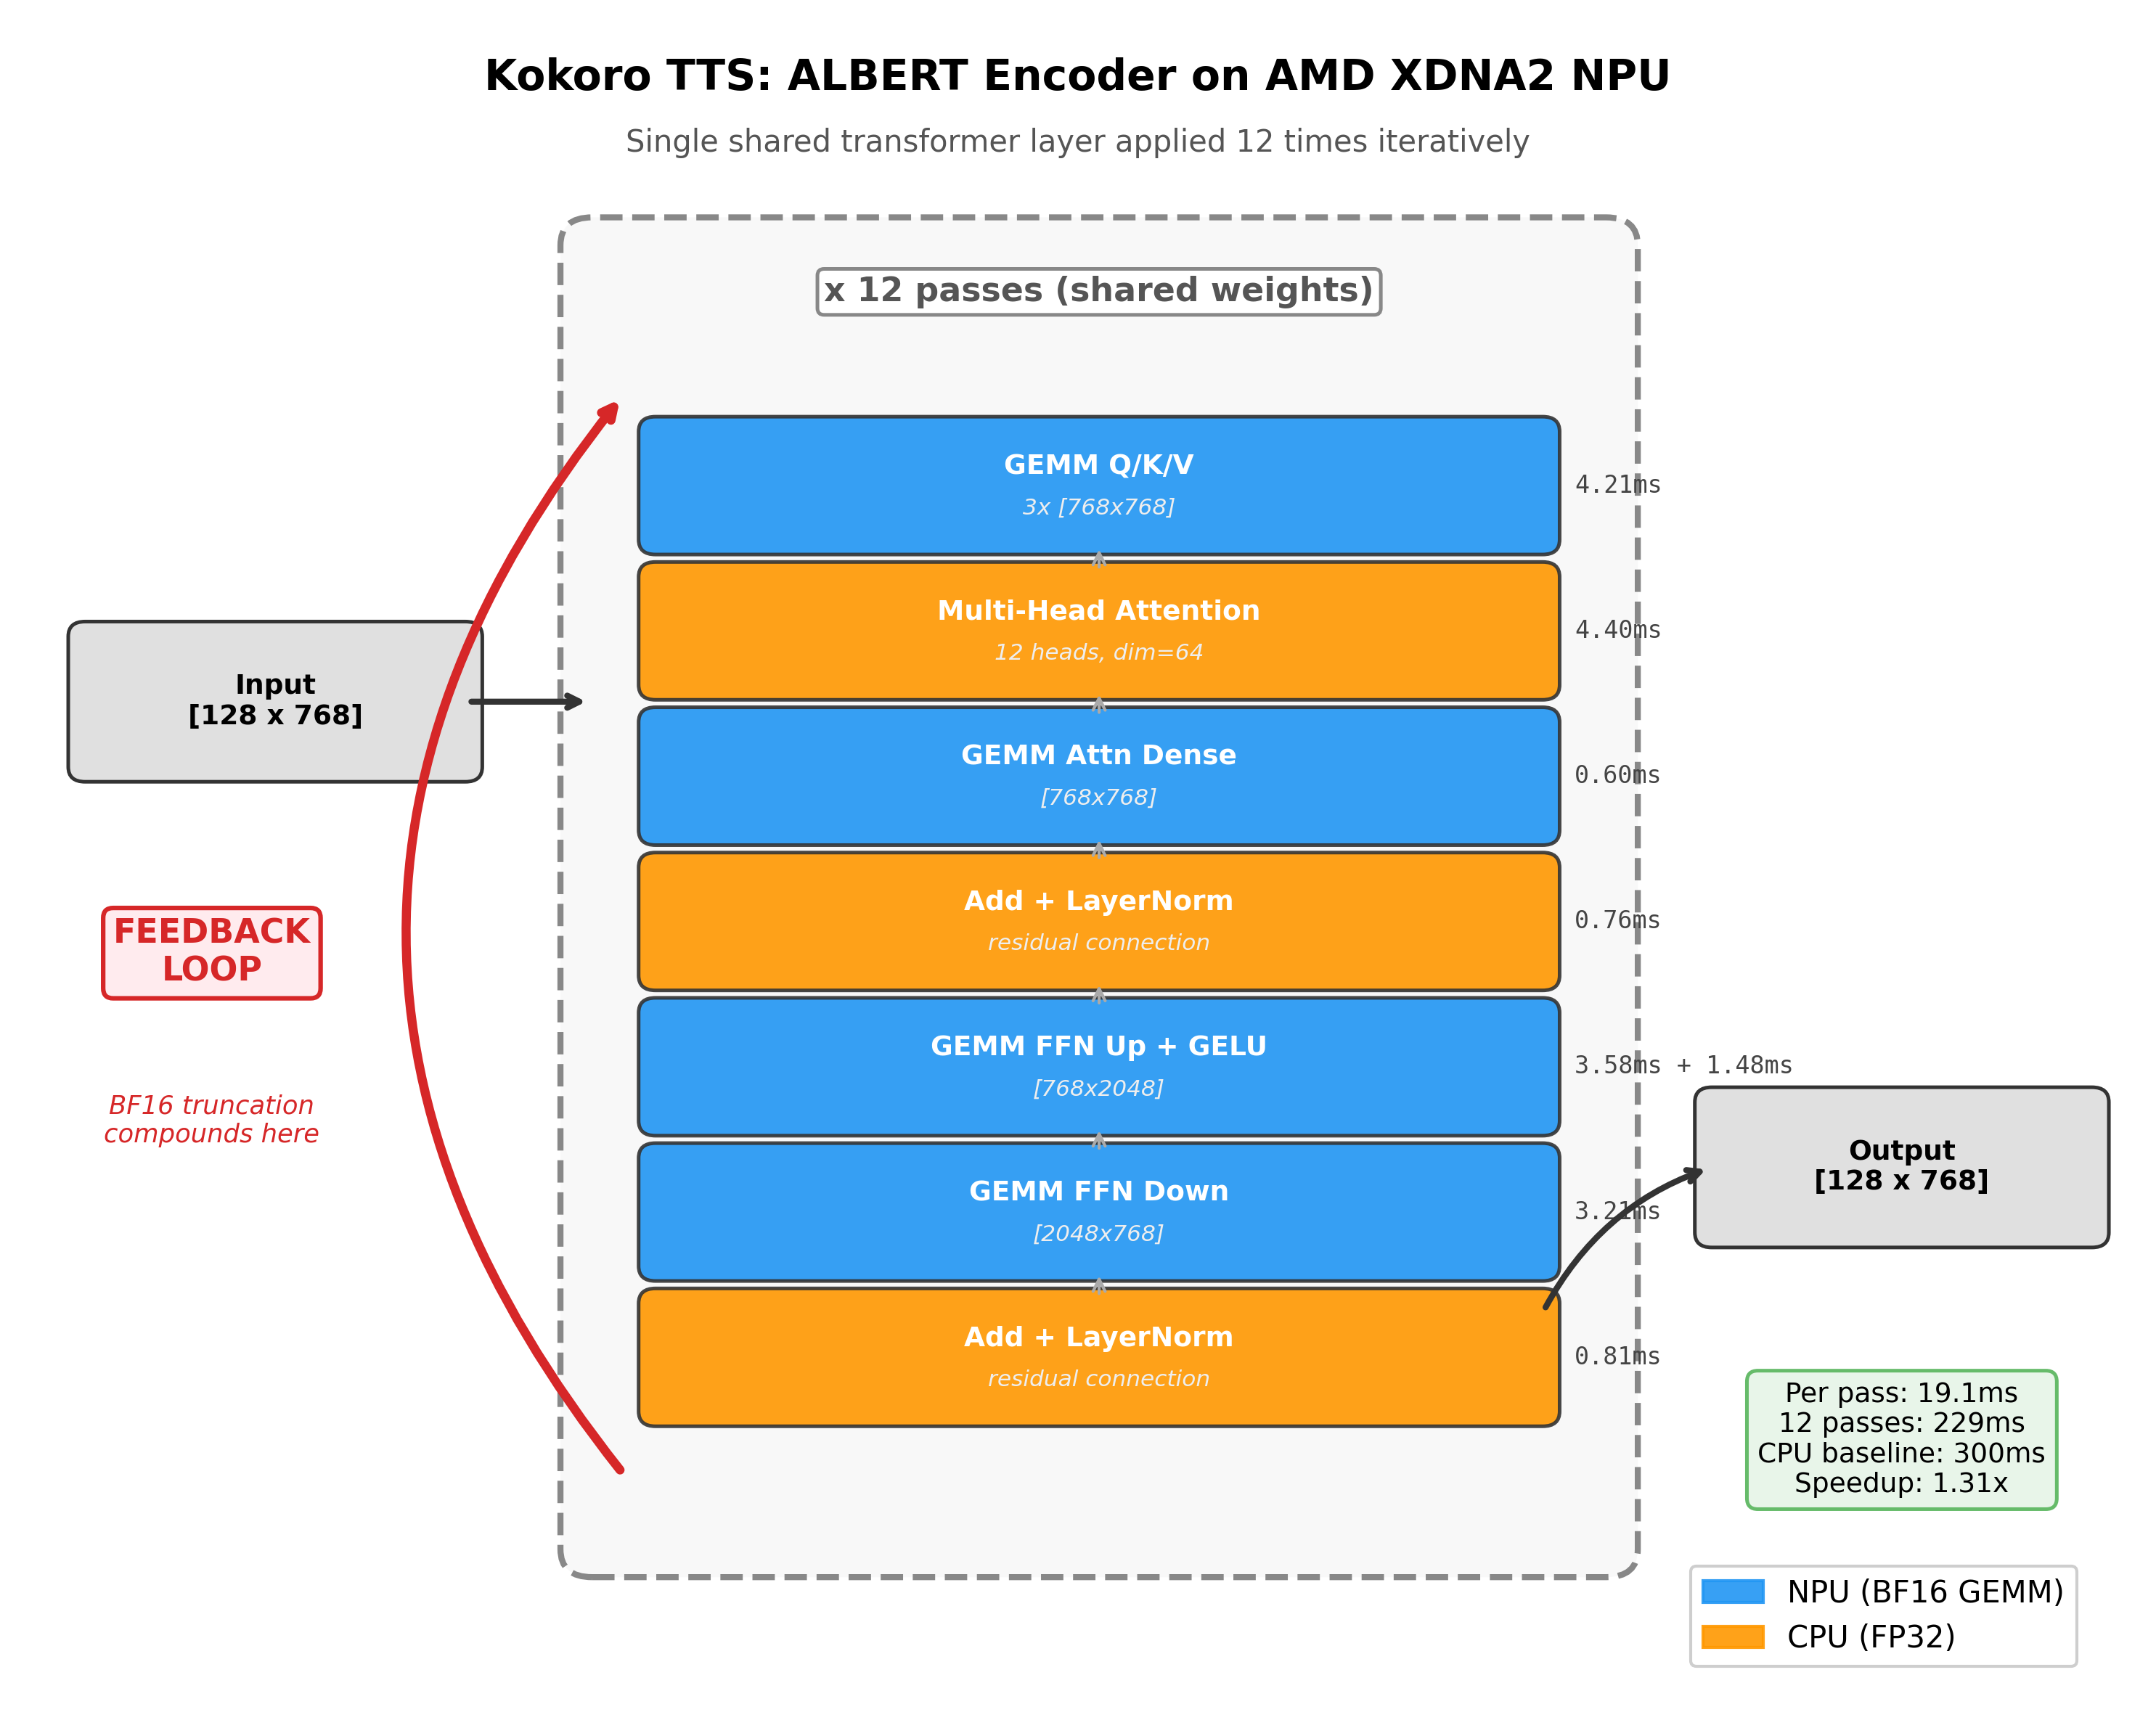
\includegraphics[width=\linewidth]{figures/fig1_architecture.png}
    \caption{ALBERT encoder architecture with NPU/CPU device mapping. Blue blocks execute on the NPU via BF16 GEMM; orange blocks run on CPU in FP32. The red feedback arrow marks the iterative path where BF16 truncation compounds.}
    \label{fig:architecture}
\end{figure}

IRON GEMM achieves 248$\times$ speedup over our initial custom kernel (0.32\,ms vs.\ 79.5\,ms for $128{\times}768{\times}768$), reaching 475--910\,GFLOPS depending on matrix dimensions---approaching peak throughput for memory-bandwidth-bound workloads at 0.42\,ops/byte arithmetic intensity.

The full ALBERT benchmark progressed through six optimization steps (Table~\ref{tab:optimization}, Figure~\ref{fig:trajectory}).

\begin{table}[t]
\centering
\caption{Optimization trajectory for 12-pass ALBERT on XDNA2 NPU.}
\label{tab:optimization}
\small
\begin{tabular}{@{}clcc@{}}
\toprule
Step & Change & Latency (ms) & vs.\ CPU \\
\midrule
1 & Custom 4-tile GEMM + per-head MHA & 1022 & 3.4$\times$ slower \\
2 & IRON GEMM + IRON MHA & 261 & 1.15$\times$ faster \\
3 & Buffer reuse + fast GELU & 184 & 1.63$\times$ faster \\
4 & Real weights + POST-norm & 246 & 1.22$\times$ faster \\
5 & Fused QKV GEMM & 243 & 1.24$\times$ faster \\
6 & AVX2 CPU MHA (precision fix) & 229 & 1.31$\times$ faster \\
\bottomrule
\end{tabular}
\end{table}

The step 3-to-4 regression is expected: random weights undercount real data movement, and the correct POST-norm architecture includes an attention output dense GEMM absent from earlier estimates.

\begin{figure}[t]
    \centering
    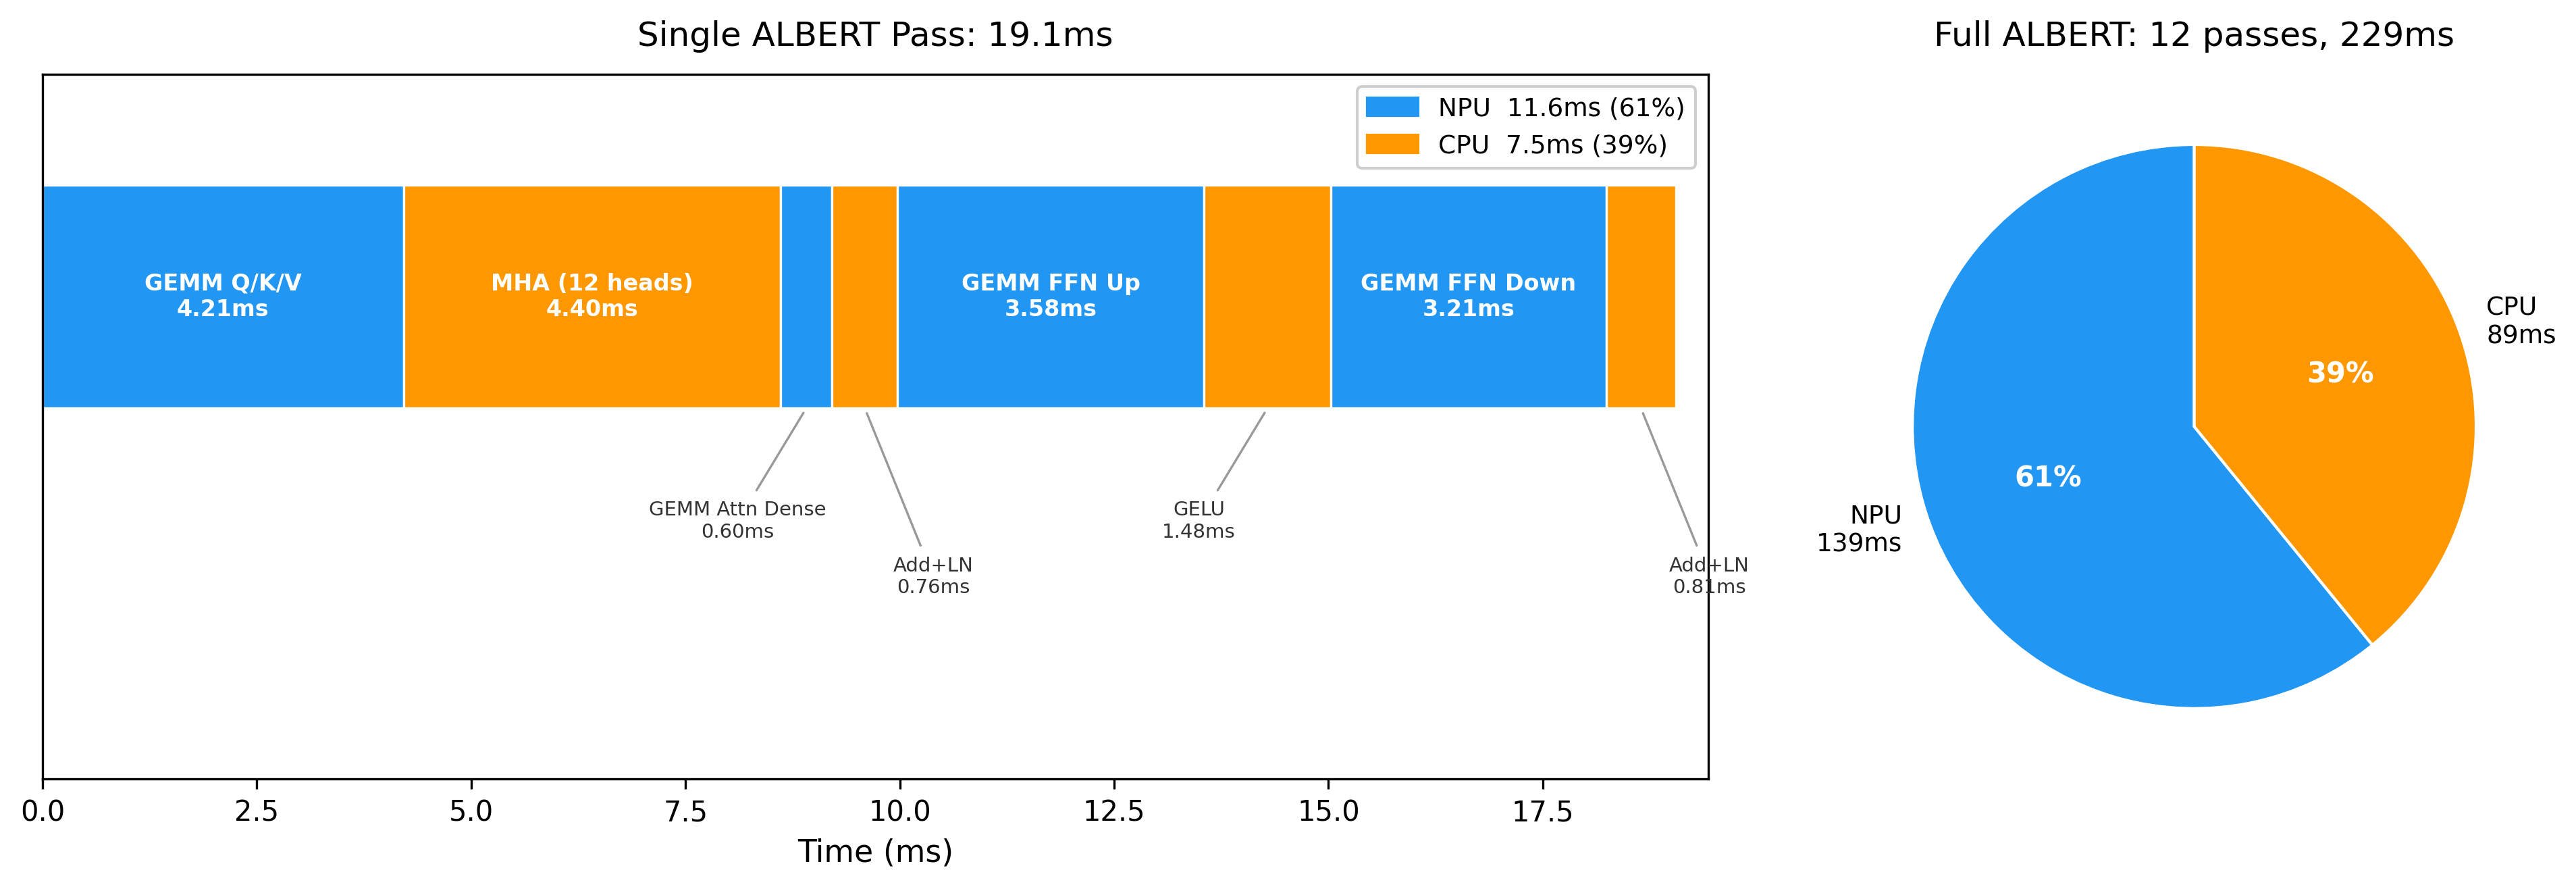
\includegraphics[width=\linewidth]{figures/fig2_timing_breakdown.png}
    \caption{Per-pass timing breakdown (left) and device split for full 12-pass ALBERT (right). NPU operations (GEMMs) account for 61\% of execution time.}
    \label{fig:breakdown}
\end{figure}

The final configuration (229\,ms) breaks down per-pass as shown in Figure~\ref{fig:breakdown}: GEMM Q/K/V (4.21\,ms), MHA (4.40\,ms), GEMM Attn Dense (0.60\,ms), Add+LayerNorm (0.76\,ms), GEMM FFN Up (3.58\,ms), GELU (1.48\,ms), GEMM FFN Down (3.21\,ms), Add+LayerNorm (0.81\,ms). All GEMMs are firmly \textbf{memory-bandwidth-bound} (0.42\,ops/byte against ${\sim}51$\,GB/s DDR bandwidth).

\subsection{Precision Degradation}
\label{sec:precision}

Figure~\ref{fig:precision} shows the central finding: correlation vs.\ FP32 reference degrades across ALBERT's 12 passes at rates that vary dramatically by configuration.

\begin{figure}[t]
    \centering
    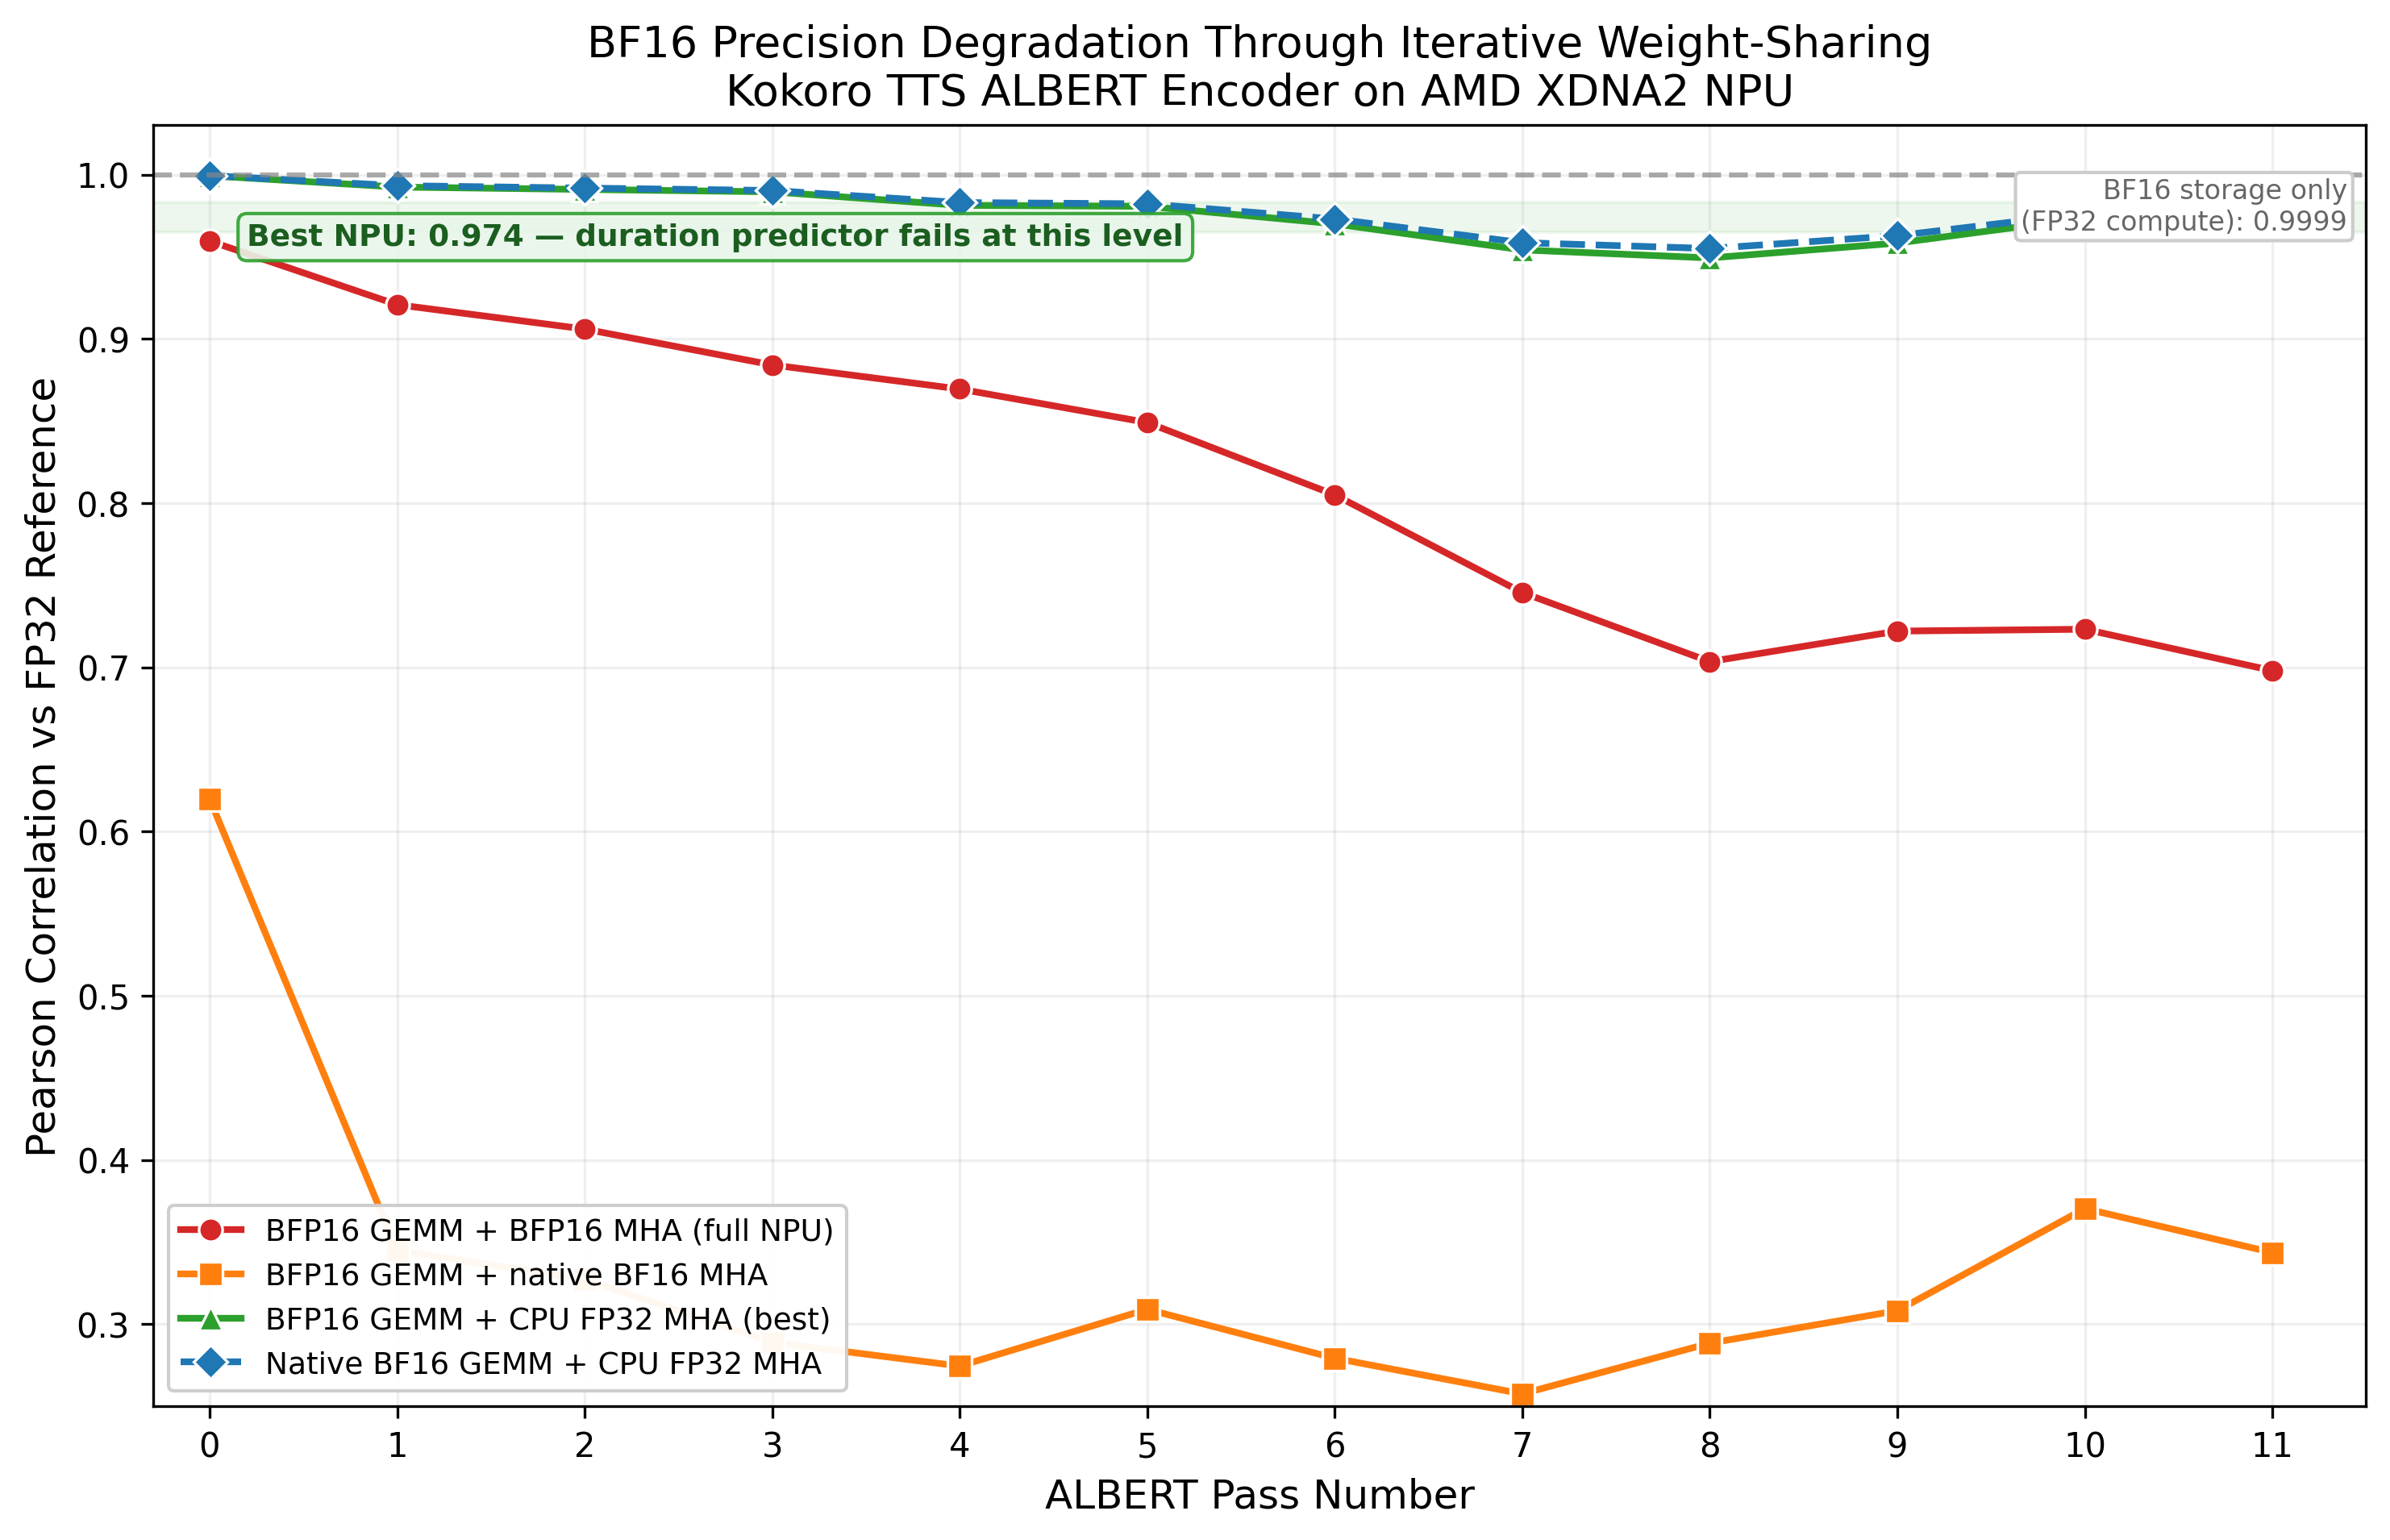
\includegraphics[width=\linewidth]{figures/fig3_precision_curve.png}
    \caption{Per-pass Pearson correlation vs.\ FP32 reference across 12 ALBERT passes. Four configurations shown: full NPU (red), native BF16 MHA (orange), best hybrid with CPU MHA (green), and native BF16 GEMM with CPU MHA (blue). The BF16 storage-only baseline (0.9999, dashed gray) confirms that storage format is benign; the error is in GEMM \emph{compute} truncation.}
    \label{fig:precision}
\end{figure}

\begin{table}[t]
\centering
\caption{Configuration comparison: final ALBERT output correlation, latency, and audio quality.}
\label{tab:precision}
\small
\begin{tabular}{@{}lccc@{}}
\toprule
Configuration & Correlation & Latency (ms) & Audio \\
\midrule
BFP16 GEMM + BFP16 MHA & 0.698 & 244 & Destroyed \\
BFP16 GEMM + Native BF16 MHA & 0.343 & 275 & Destroyed \\
BFP16 GEMM + CPU FP32 MHA & 0.974 & 229 & Duration mismatch \\
Native BF16 GEMM + CPU FP32 MHA & 0.974 & 266 & Duration mismatch \\
BF16-simulated CPU (storage only) & 0.9999 & --- & Fine \\
FP32 CPU (reference) & 1.000 & ${\sim}$300 & Reference \\
\bottomrule
\end{tabular}
\end{table}

The configuration comparison (Table~\ref{tab:precision}, Figure~\ref{fig:waterfall}) isolates three independent error sources:

\begin{figure}[t]
    \centering
    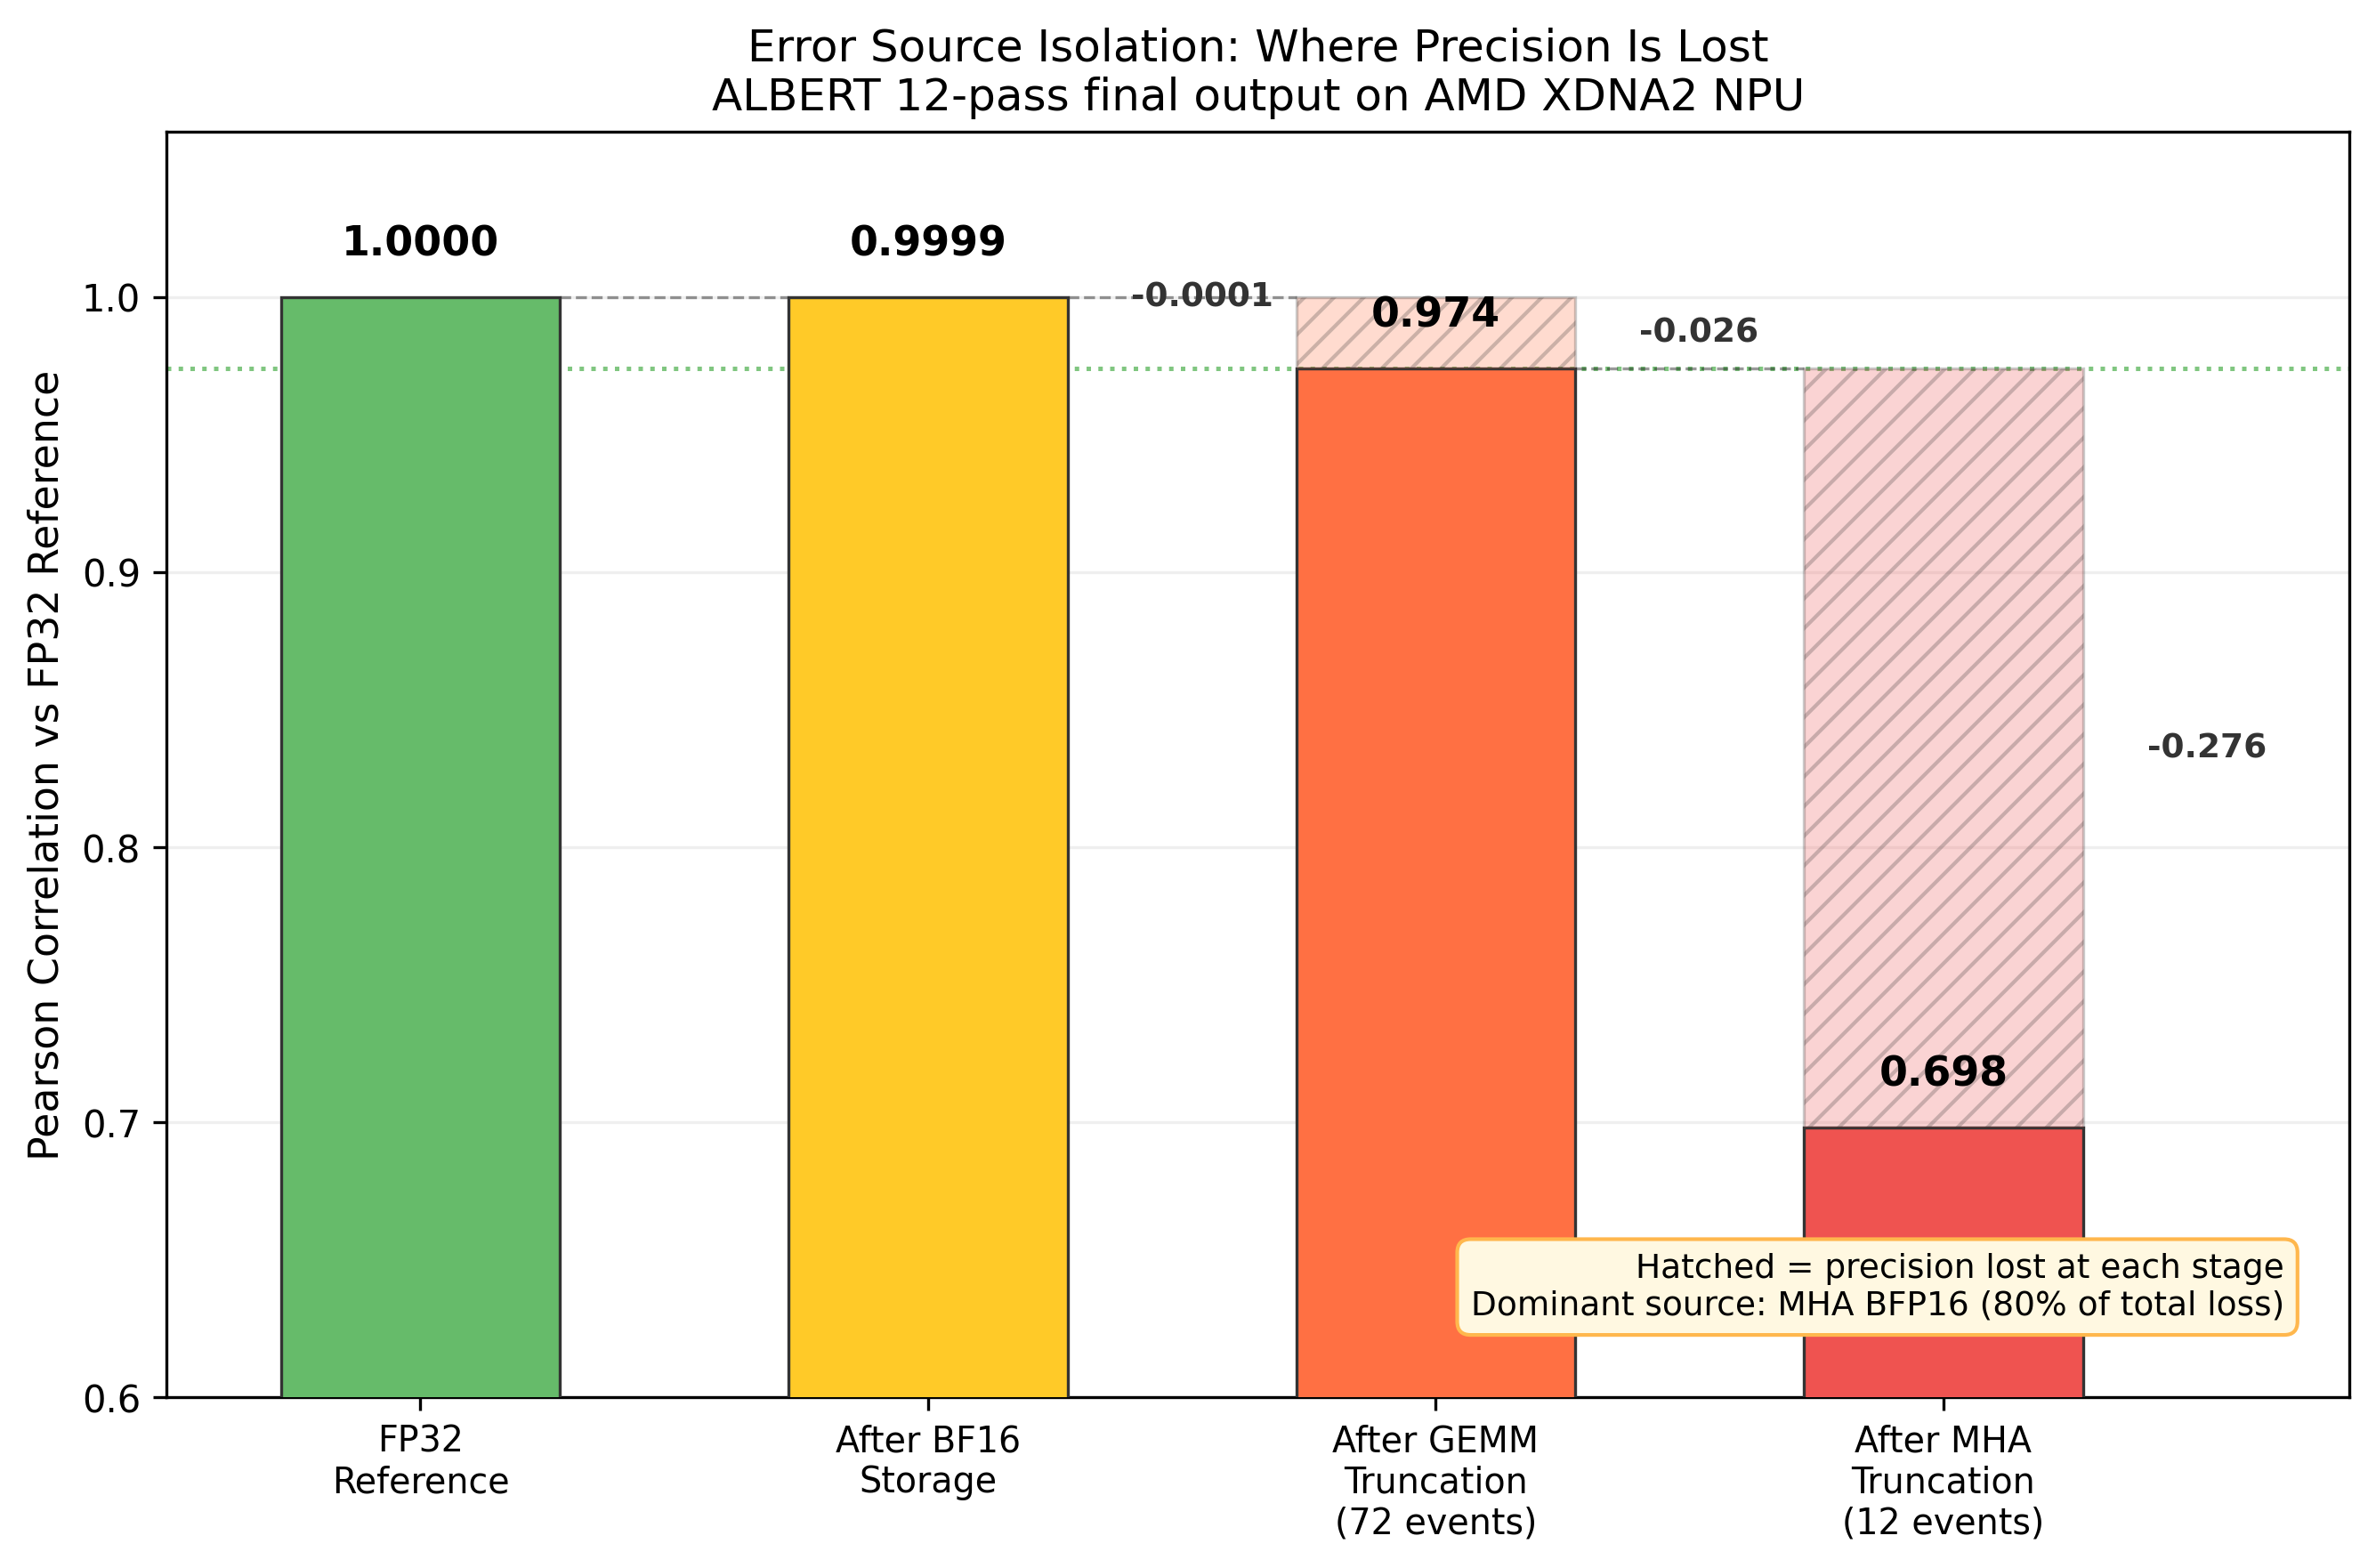
\includegraphics[width=0.85\linewidth]{figures/fig4_error_waterfall.png}
    \caption{Error source waterfall: cumulative precision loss from FP32 reference (1.000) through BF16 storage ($-0.0001$), GEMM input truncation ($-0.026$), and MHA BFP16 truncation ($-0.276$). MHA accounts for 80\% of total precision loss.}
    \label{fig:waterfall}
\end{figure}

\textbf{MHA is the dominant error source.} Replacing only MHA with CPU FP32 (keeping BFP16 GEMM on NPU) raises correlation from 0.698 to 0.974---larger than any GEMM-side change.

\textbf{BFP16 is paradoxically better than native BF16 for MHA.} Native BF16 MHA (element-wise truncation) yields 0.343 correlation---far worse than BFP16 MHA's 0.698. BFP16's shared exponent preserves relative magnitudes within attention score blocks, while element-wise BF16 independently distorts each score, destroying the softmax distribution more severely.

\textbf{GEMM truncation creates an irreducible 0.974 ceiling.} Both BFP16 and native BF16 GEMM yield identical 0.974 correlation when MHA runs on CPU. The BF16-simulated CPU test (0.9999) confirms that BF16 storage between passes is benign---the problem is BF16 truncation at GEMM \emph{inputs}.

\subsection{Audio Impact}

\begin{figure}[t]
    \centering
    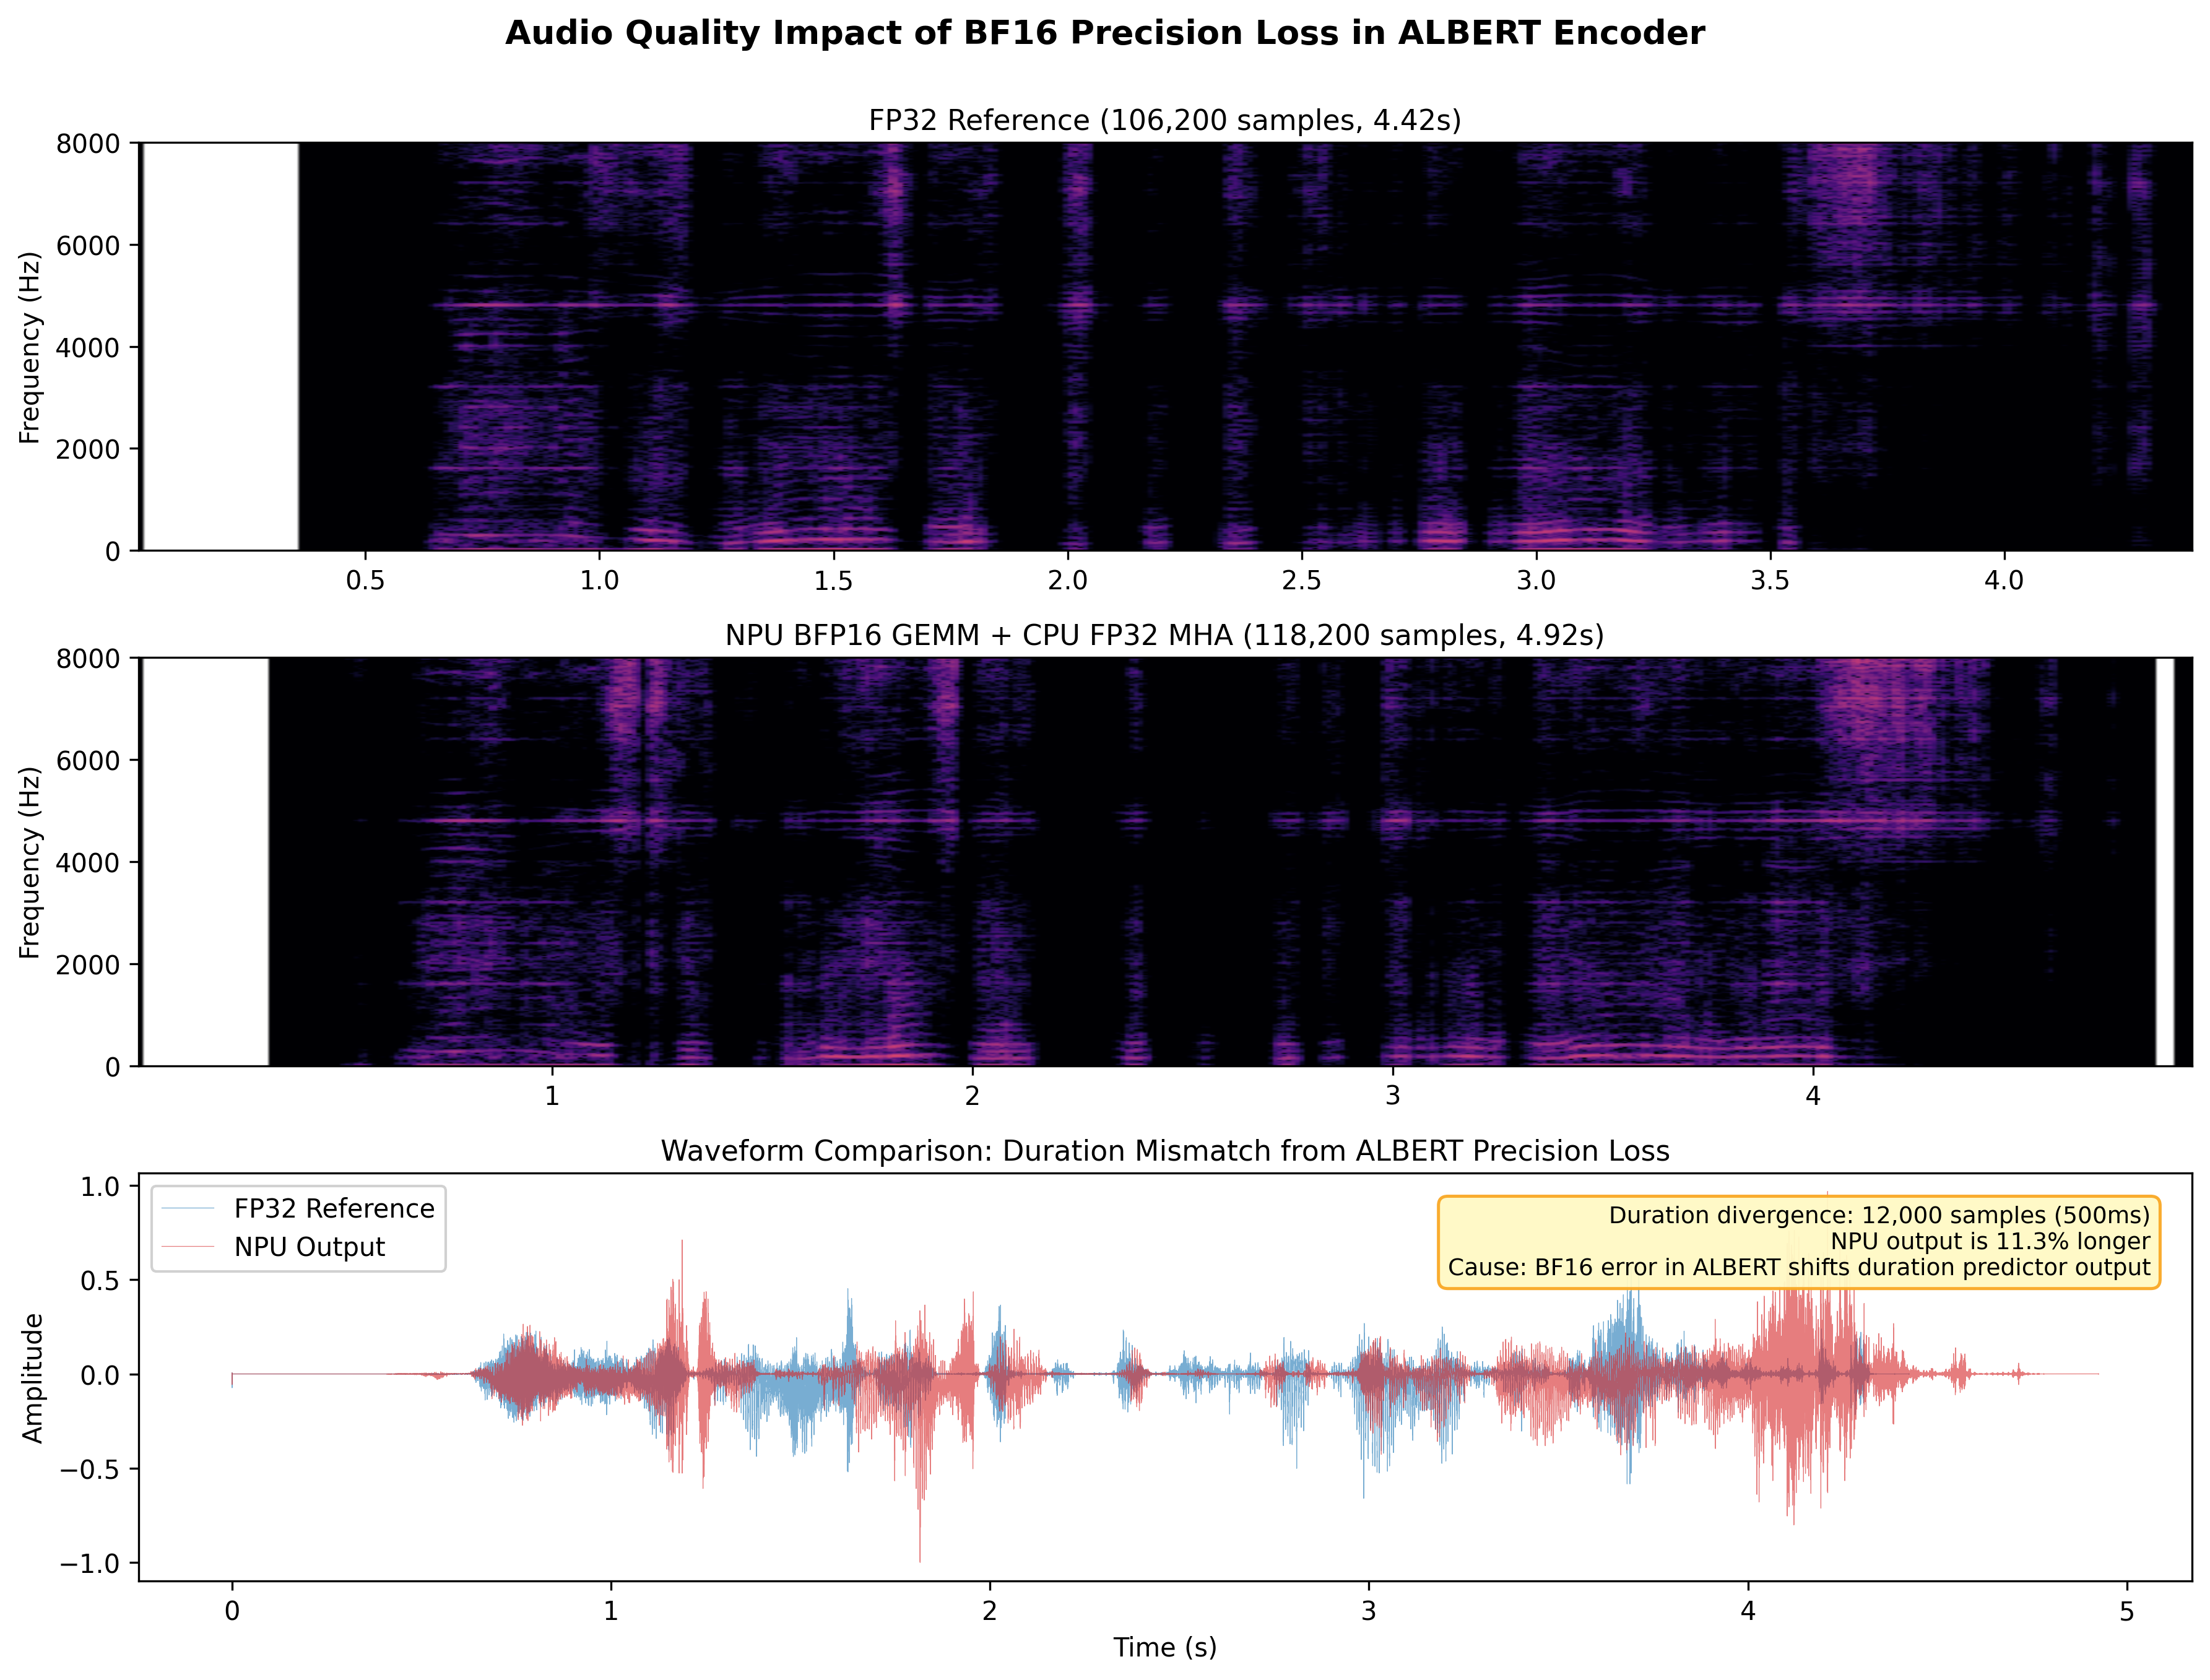
\includegraphics[width=\linewidth]{figures/fig5_spectrograms.png}
    \caption{Spectrogram and waveform comparison between FP32 reference (106,200 samples, 4.42\,s) and best NPU configuration (118,200 samples, 4.92\,s). The 11.3\% duration mismatch is caused by ALBERT precision loss affecting the downstream duration predictor.}
    \label{fig:spectrograms}
\end{figure}

The 0.974 correlation ceiling sounds numerically high but is functionally insufficient. Kokoro's duration predictor---a stack of 6 LSTMs---is highly sensitive to distributional shift in its input.

At 0.974 correlation, phoneme durations diverge enough to produce audio of a different total length: 118,200 samples (4.92\,s) vs.\ 106,200 samples (4.42\,s)---an \textbf{11.3\% duration mismatch} (Figure~\ref{fig:spectrograms}). The resulting audio has waveform correlation of 0.01 (uncorrelated due to misalignment), SNR of $-10.5$\,dB, and different prosody---unusable as a drop-in replacement. For the full-NPU configuration (0.698): audio is unintelligible.

The duration predictor acts as an \textbf{error amplifier}: continuous distributional shifts in the 768-dim hidden state are converted into discrete frame-count differences that cascade into large waveform divergence. A 2.6\% average per-dimension error is sufficient to flip discrete duration predictions.

\subsection{INT8 Quantization}

We evaluated INT8 quantization using AMD Quark~0.11.1 with text-based calibration (30 real sentences). Full INT8 produced $-15.6$\,dB SNR; selective INT8 (ALBERT in FP32, decoder/vocoder in INT8) produced $-16.8$\,dB---\emph{worse}. This demonstrates that Kokoro is precision-sensitive across the \textbf{entire pipeline}, not just the iterative ALBERT encoder.

% ============================================================
\section{Analysis}

\subsection{Why Iterative Architectures Amplify BF16 Error}

Consider a single ALBERT pass with 6 GEMMs, each truncating FP32 inputs to BF16 (relative error ${\sim}2^{-8}$). Over 12 passes, this yields 72 truncation events.

In a standard 12-layer transformer with independent weights, each layer projects into a different subspace. Truncation errors at layer $i$ are not aligned with layer $i{+}1$'s principal components, yielding $\mathcal{O}(\sqrt{72}) \approx 8.5\times$ the single-GEMM error.

In ALBERT, the same weights are applied 12 times. Errors aligned with dominant eigenvectors are amplified at each pass. Instead of random-walk accumulation, error follows the weight matrix's spectral structure, growing as $\mathcal{O}(N)$ or worse for aligned components. The partial recovery after pass~7 (Figure~\ref{fig:precision}) is attributed to LayerNorm re-centering---but LayerNorm corrects scale and offset, not representation \emph{direction}.

\subsection{The Duration Predictor as Error Amplifier}

The duration predictor converts continuous 768-dim representations into discrete per-phoneme frame counts. This discretization acts as a hard nonlinearity: a continuous error of $\epsilon$ can produce a discrete change of $\geq$1 frame for phonemes near integer boundaries. Across 20--50 phonemes per utterance, even low per-phoneme error probability accumulates into significant total duration change. Our observed 11.3\% mismatch (12,000 samples at 24\,kHz) represents ${\sim}$0.5 frames/phoneme shift.

\textbf{Implication:} Precision requirements must be evaluated at the full pipeline level, not just the accelerated component. The 0.974 correlation appears adequate in isolation but fails the downstream LSTM predictor.

\subsection{Implications Beyond Kokoro}

Our findings generalize to any architecture iteratively applying shared weights through BF16-only hardware:

\begin{itemize}[nosep]
    \item \textbf{Diffusion models} (16--50 denoising steps through shared UNet): same compounding mechanism, though noise-to-signal convergence may partially decorrelate early-step errors.
    \item \textbf{Universal Transformers}~\citep{dehghani2019universal}: identical weight-sharing pattern; our results predict degradation at depth $\geq$12.
    \item \textbf{Iterative refinement networks}: equilibrium networks, DEQ models, iterative amortized inference.
\end{itemize}

This is not AMD-specific. Any hardware with BF16-only matrix inputs (certain TPU configurations, custom ASICs) faces the same constraint.

\subsection{When BF16 NPU Inference Works Well}

BF16 precision is adequate for: (1)~standard transformers with independent layer weights (LIRA~\citep{lira2025} demonstrates Whisper on XDNA2); (2)~convolutional networks without weight sharing; (3)~shallow iteration ($\leq$3 passes) with tolerant downstream consumers.

\begin{figure}[t]
    \centering
    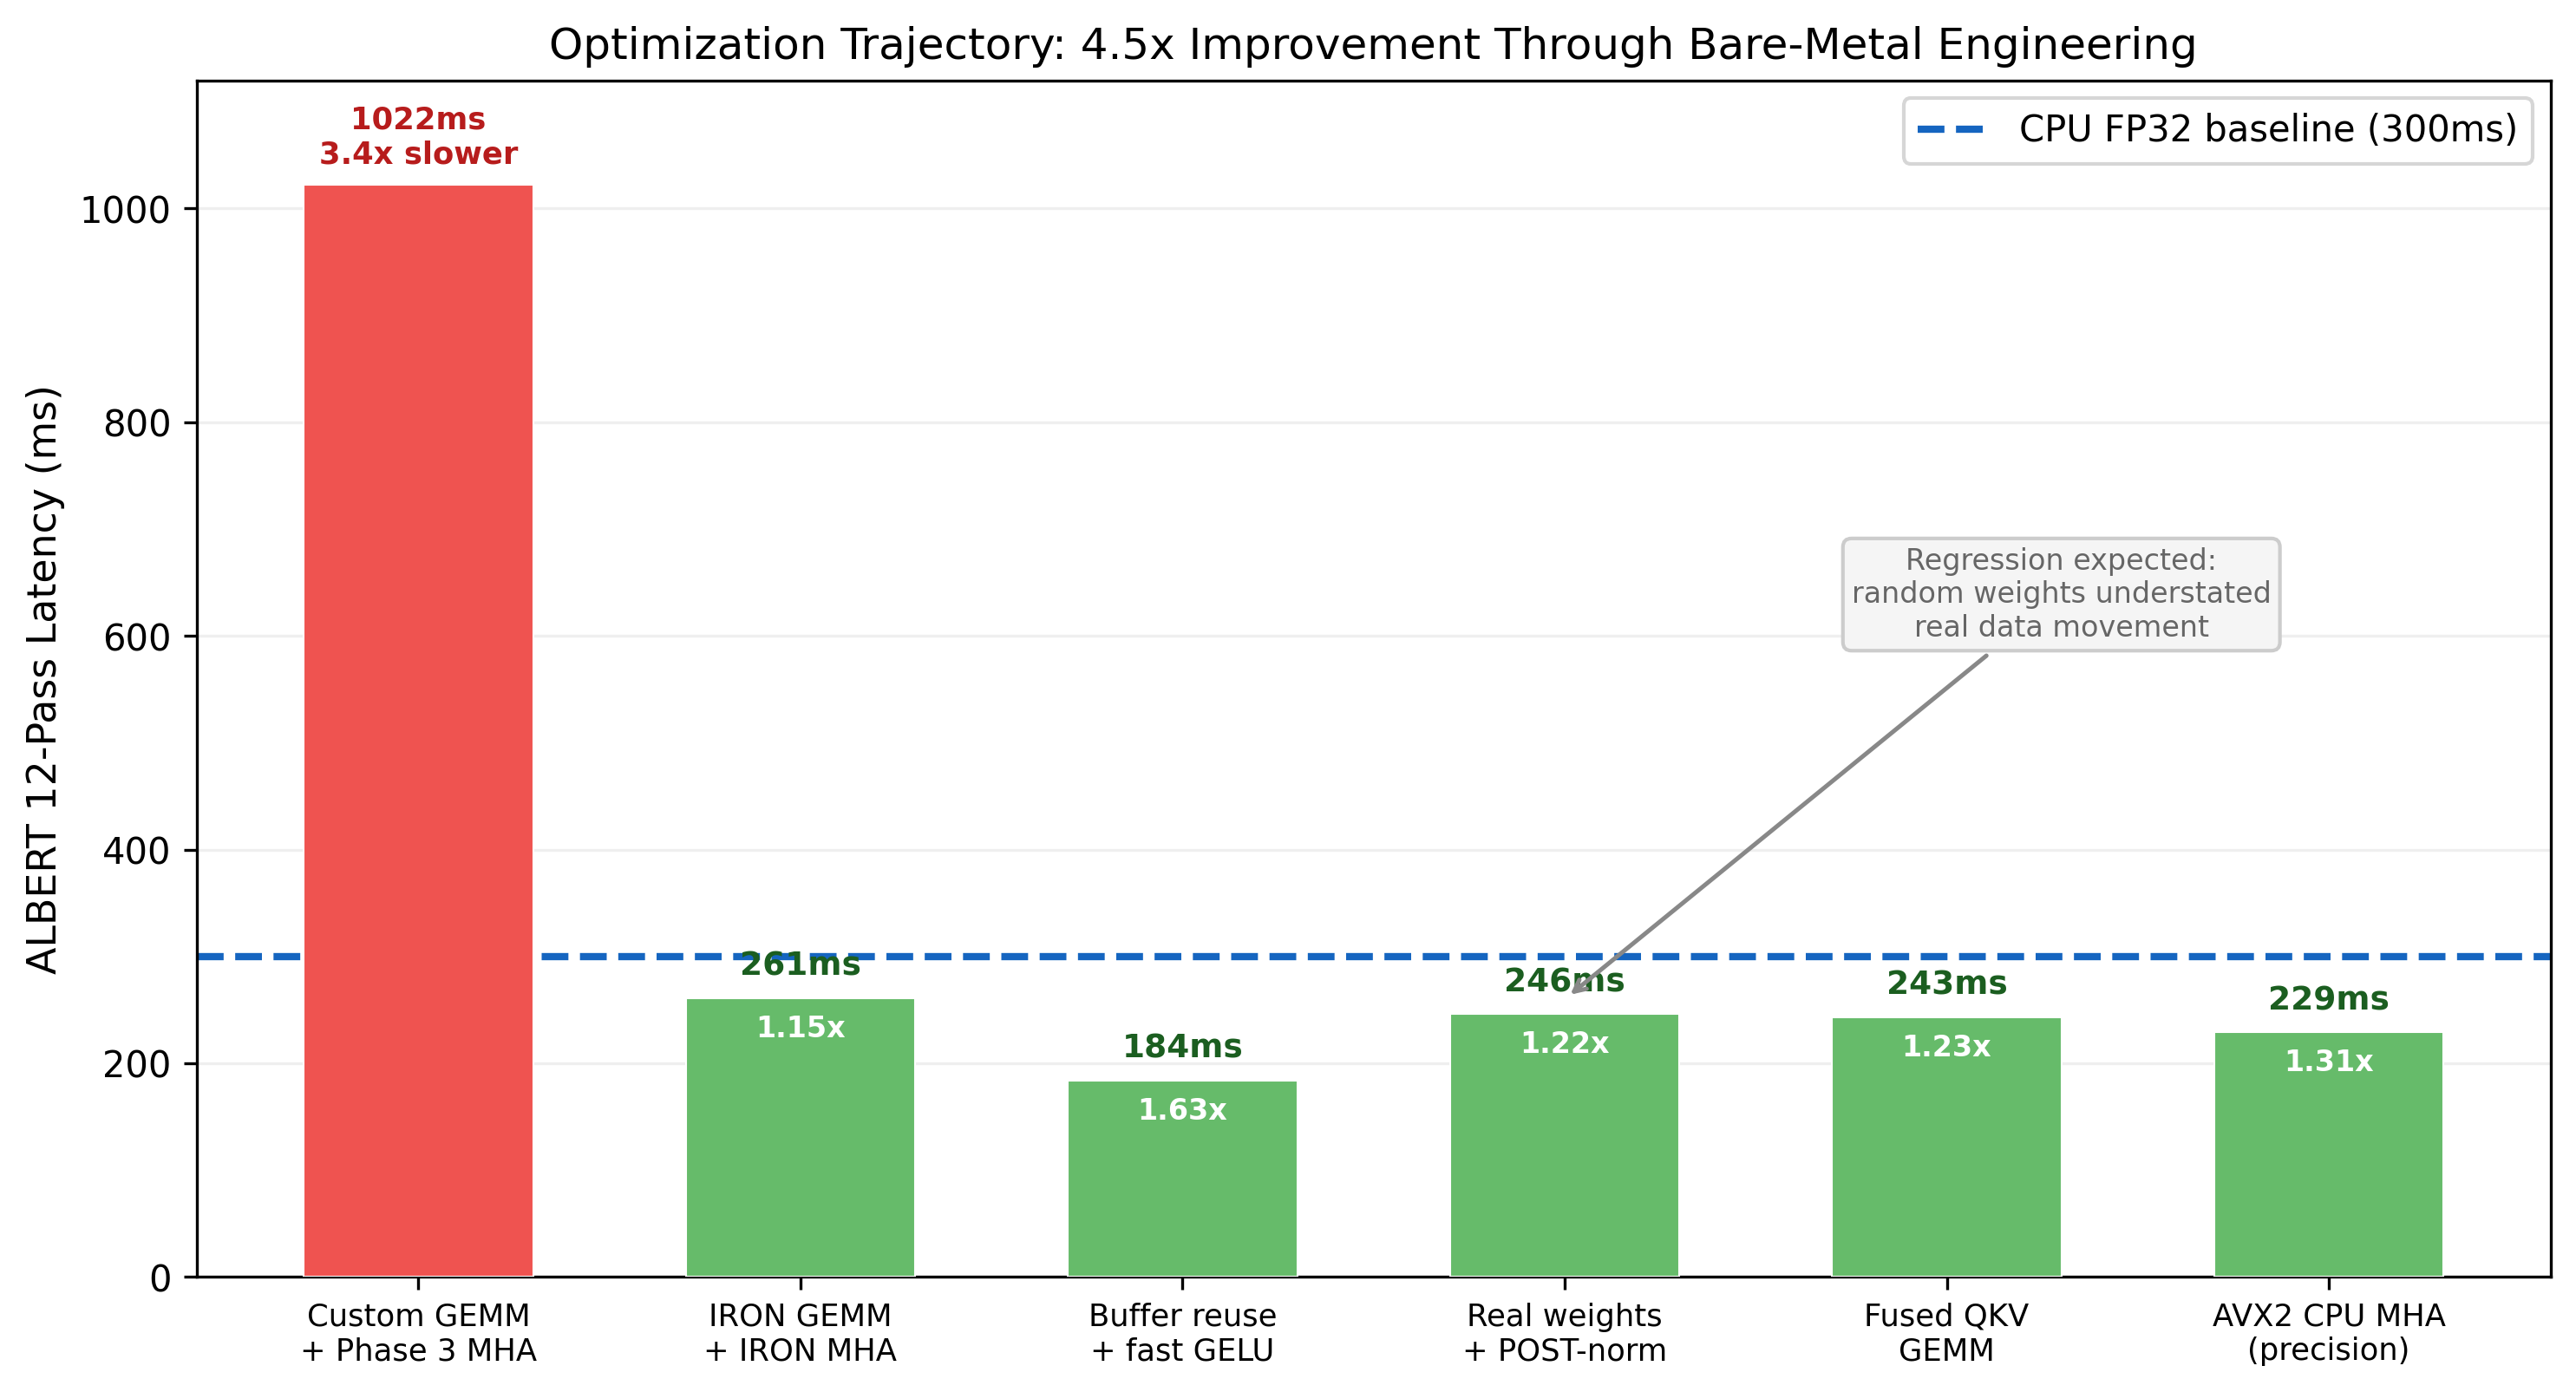
\includegraphics[width=\linewidth]{figures/fig6_optimization_trajectory.png}
    \caption{Optimization trajectory: 4.5$\times$ improvement from naive NPU implementation (1022\,ms) to final configuration (229\,ms) through six engineering steps.}
    \label{fig:trajectory}
\end{figure}

% ============================================================
\section{Related Work}

\textbf{NPU inference.} LIRA~\citep{lira2025} demonstrates Whisper ASR on XDNA2 using VitisAI with the encoder's homogeneous architecture. GPT-SoVITS on XDNA1 was 2--3$\times$ slower than CPU due to fragmentation. To our knowledge, no prior work characterizes BF16 precision through iterative architectures on bare-metal NPU hardware.

\textbf{Quantization for TTS.} Our Quark INT8 results ($-15.6$\,dB SNR) extend prior observations of Kokoro's precision sensitivity to the entire pipeline.

\textbf{ALBERT precision.} The original ALBERT paper~\citep{lan2020albert} does not discuss reduced-precision inference. Recent work on analog computing~\citep{aguirre2025albert} explores weight-sharing on different hardware but does not characterize precision compounding.

\textbf{BF16 error analysis.} Prior work focuses on training stability~\citep{kalamkar2019bf16}, where stochastic rounding provides natural error decorrelation. Inference through iterative architectures lacks these corrective mechanisms.

\textbf{Bare-metal NPU.} IRON~\citep{iron2024} provides the programming model; prior work focuses on operator-level benchmarks. We extend to a complete multi-operation workload with real weights.

% ============================================================
\section{Conclusion}

We have demonstrated that BF16 input truncation in NPU matrix units compounds through iterative weight-sharing architectures, producing outputs that are numerically close (0.974 correlation) but functionally unusable for sensitive downstream consumers. The error mechanism---correlated amplification through shared weight matrices---is fundamental to the interaction between limited-precision hardware and iterative computation.

Our bare-metal XDNA2 characterization shows that performance is achievable (1.31$\times$ CPU speedup, 229\,ms through 4.5$\times$ optimization), but the precision ceiling is the binding constraint. The practical recommendation is to run iterative components on CPU and target NPU acceleration at single-pass stages.

For hardware designers: adding an FP32 input path to the matrix multiply unit would unlock iterative architectures without sacrificing single-pass throughput. For model designers: BF16-aware training with quantization noise injection during iterative passes could produce robust models, though this requires deployment-target awareness during training.

All code, raw data, and analysis tools are available at \url{https://github.com/syntax1killer/npu-tts-research}.

% ============================================================
\begin{thebibliography}{8}

\bibitem[Lan et~al.(2020)]{lan2020albert}
Z.~Lan, M.~Chen, S.~Goodman, K.~Gimpel, P.~Sharma, and R.~Soricut.
\newblock {ALBERT}: A lite {BERT} for self-supervised learning of language representations.
\newblock In \emph{ICLR}, 2020.

\bibitem[Ho et~al.(2020)]{ho2020denoising}
J.~Ho, A.~Jain, and P.~Abbeel.
\newblock Denoising diffusion probabilistic models.
\newblock In \emph{NeurIPS}, 2020.

\bibitem[Dehghani et~al.(2019)]{dehghani2019universal}
M.~Dehghani, S.~Gouws, O.~Vinyals, J.~Uszkoreit, and {\L}.~Kaiser.
\newblock Universal transformers.
\newblock In \emph{ICLR}, 2019.

\bibitem[Hexgrad(2024)]{kokoro2024}
Hexgrad.
\newblock Kokoro {TTS}.
\newblock \url{https://huggingface.co/hexgrad/Kokoro-82M}, 2024.

\bibitem[AMD(2024)]{iron2024}
AMD.
\newblock {IRON}: Close-to-metal programming for {AI} engine.
\newblock \url{https://github.com/amd/IRON}, 2024.

\bibitem[AMD(2025)]{lira2025}
AMD.
\newblock {LIRA}: Leveraging intelligence with {Ryzen AI}.
\newblock \url{https://github.com/amd/LIRA}, 2025.

\bibitem[Aguirre et~al.(2025)]{aguirre2025albert}
M.~Aguirre et~al.
\newblock {ALBERT} on analog in-memory computing.
\newblock \emph{Nature Communications}, 2025.

\bibitem[Kalamkar et~al.(2019)]{kalamkar2019bf16}
P.~Kalamkar et~al.
\newblock A study of {BFLOAT16} for deep learning training.
\newblock \emph{arXiv:1905.12322}, 2019.

\end{thebibliography}

\end{document}
